\documentclass{article}

% Language setting
% Replace `english' with e.g. `spanish' to change the document language
\usepackage[english]{babel}

% Set page size and margins
% Replace `letterpaper' with `a4paper' for UK/EU standard size
\usepackage[letterpaper,top=2cm,bottom=2cm,left=3cm,right=3cm,marginparwidth=1.75cm]{geometry}

% Useful packages
\usepackage{amsmath}
\usepackage{graphicx}
\usepackage[colorlinks=true, allcolors=blue]{hyperref}

\title{MP2: Simple File System}
\author{Your name\\UIN: xxxxxx\\CSCE611: Operating System}

\begin{document}

\date{}
\maketitle

% \begin{abstract}
% \end{abstract}

\section*{Assigned Tasks}

\textbf{Main:} Completed. \\
\textbf{Bonus Option 1:} Completed. \\
\textbf{Bonus Option 2:} Partially completed. \\
\textbf{Bonus Option 3:} Idea is given in design doc but did not implement the code. \\
\textbf{Bonus Option 4:} Did not attempt. \\


\section*{System Design}

Describe the goal of the machine problem and how you design the system to solve the problem. Do not write the methods name or what the methods do here. Use next section for that. Rather, give an overview about how your system works and what general approaches you used. You can write this as a paragraph, use bullet points, or add pictures for the design. You can add photos of hand-drawn pictures or diagrams. No need to spend time for professionally-looking pictures. Think of this section as if you were describing the system design to your friend.

\begin{figure}[!h]
\centering
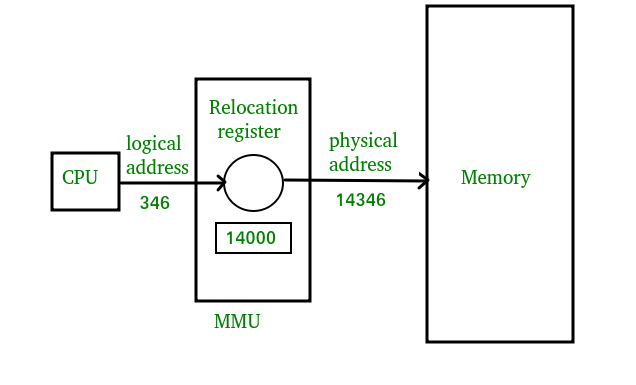
\includegraphics[width=0.8\textwidth]{figs/memory_design.png}
\caption{Memory design}
\end{figure}

\newpage
\section*{Code Description}

Describe your code setup here, any instruction about how to compile the code. For example, "I changed map.h, map.c, code.h, code.c for this machine problem. To compile the code use this and that in the kernel.c file."

\paragraph{map.c: allocate\_memory}: This method is used to allocate the memory. (Describe how you implemented the allocation. Add a screenshot of your code for this particular method.)

\begin{figure}[!h]
\centering
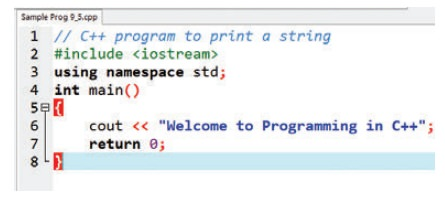
\includegraphics[width=0.3\textwidth]{figs/code_screen_shot.jpg}
\end{figure}


\paragraph{map.c: free\_memory}: Describe the method. Add a screenshot of your code for this method.

\begin{figure}[!h]
\centering
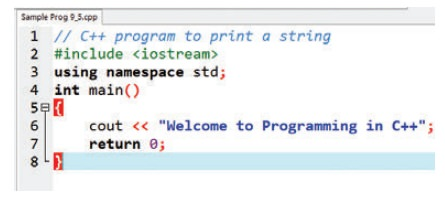
\includegraphics[width=0.3\textwidth]{figs/code_screen_shot.jpg}
\end{figure}

\section*{Bonus Option 1}
Describe how you implemented bonus option 1.

\paragraph{map.c: free\_memory}: Describe how you changed the method to accommodate for the bonus option. Add a screenshot of your code for the changed method.

\begin{figure}[!h]
\centering
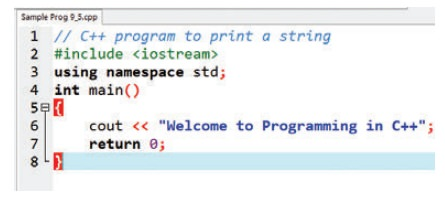
\includegraphics[width=0.3\textwidth]{figs/code_screen_shot.jpg}
\end{figure}

\section*{Bonus Option 2}
Describe how you partially complete it. What is missing? What can be added to make it work?
\section*{Bonus Option 3}
Describe your tentative approach and provide a rationale supporting your claim that it should work. What prevented you from implementing your tentative approach? 

% IMPORTANT
\section*{Testing}
{\bf This is a very important section!} Describe which efforts you have made to test your submission. Did you rely on the provided test functions? What did you add? What do you think is the coverage of your testing? What are you ignoring? (You are not expected to test improper use of your implementation. You can assume an intelligent user who uses your provided functions in the way they are supposed to be used. This assumption greatly reduces the amount of testing required.)
\end{document}